
\begin{figure}[h!]
    \caption[Net gains with the CERF burden-sharing rule.]{Net gains from the CERF burden-sharing rule in 2030. }\label{fig:gain_gdr_over_gdp_2030}
    \makebox[\textwidth][c]{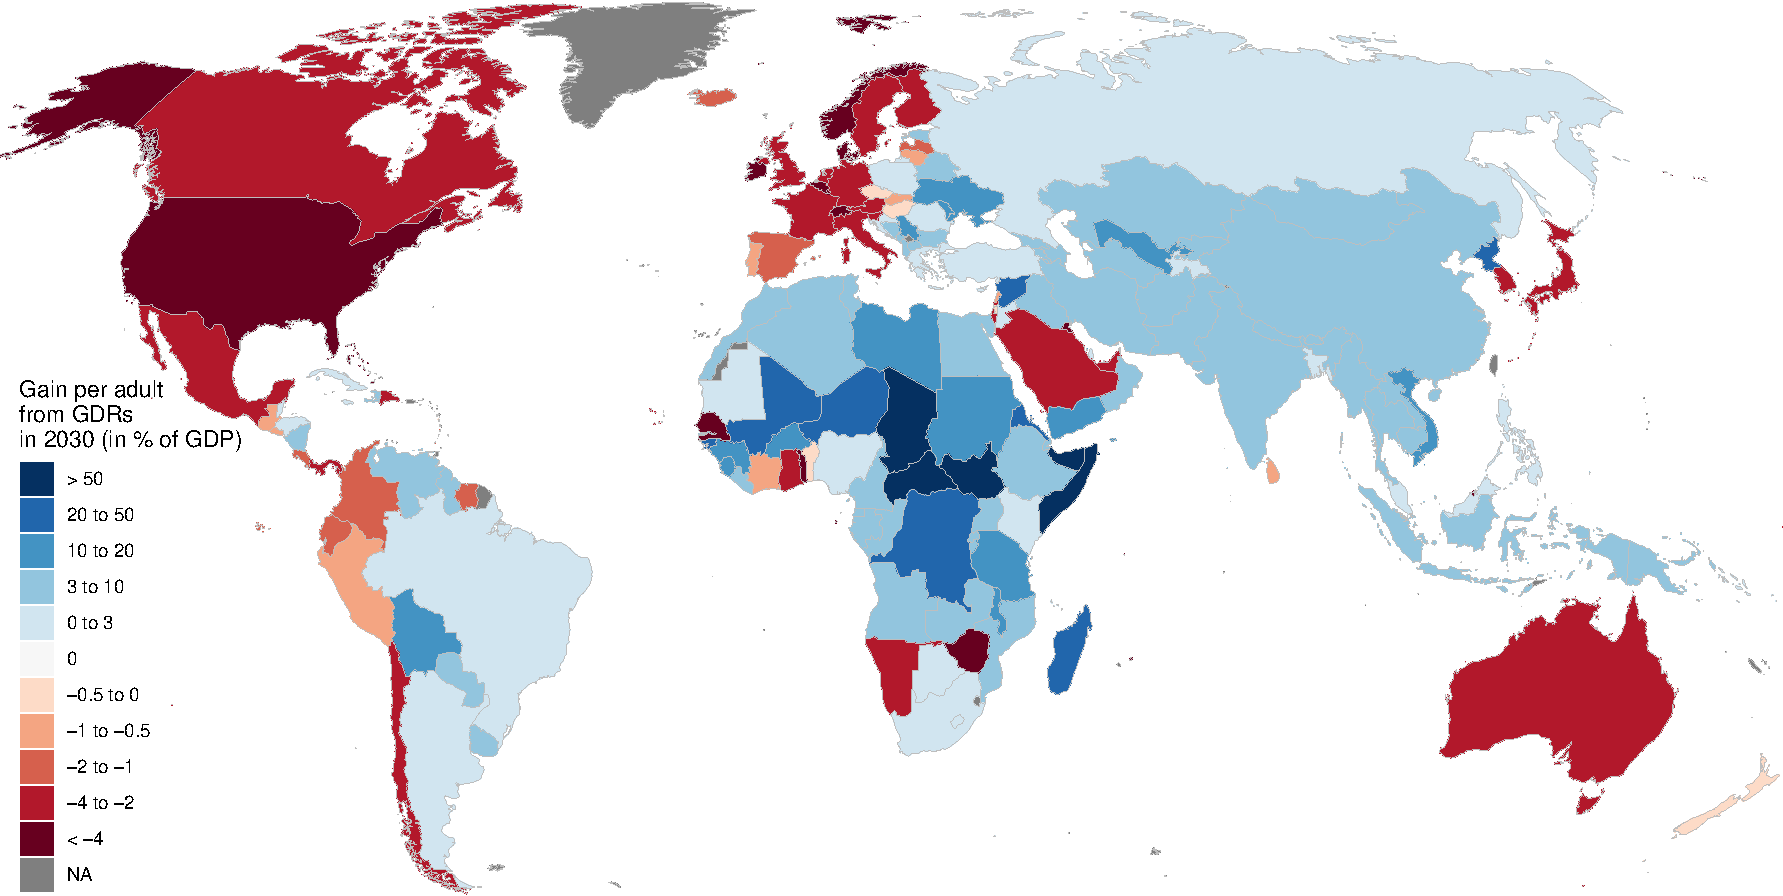
\includegraphics[width=\textwidth]{../figures/maps/gain_gdr_over_gdp_2030.pdf}} 
    {\small \textit{Note:} GDRs are calibrated with the preferred parameters of the \href{https://usfairshare.org/}{U.S. Climate Action Network} \citep{athanasiou_fair_2022} using the Efficiency scenario (2\textdegree{}C with $>$50\% chance) of the Global Energy Assessment \citep{johansson_global_2012} and a price of \$144/tCO$_\text{2}$.}
\end{figure} 

\begin{figure}[h!]
    \caption[Comparison between GDR and equal per capita burden-sharing rules.]{Difference between net gains from Greenhouse Development Rights and equal rights per capita. }\label{fig:diff_gain_gdr_gcs_over_gdp_2030}
    \makebox[\textwidth][c]{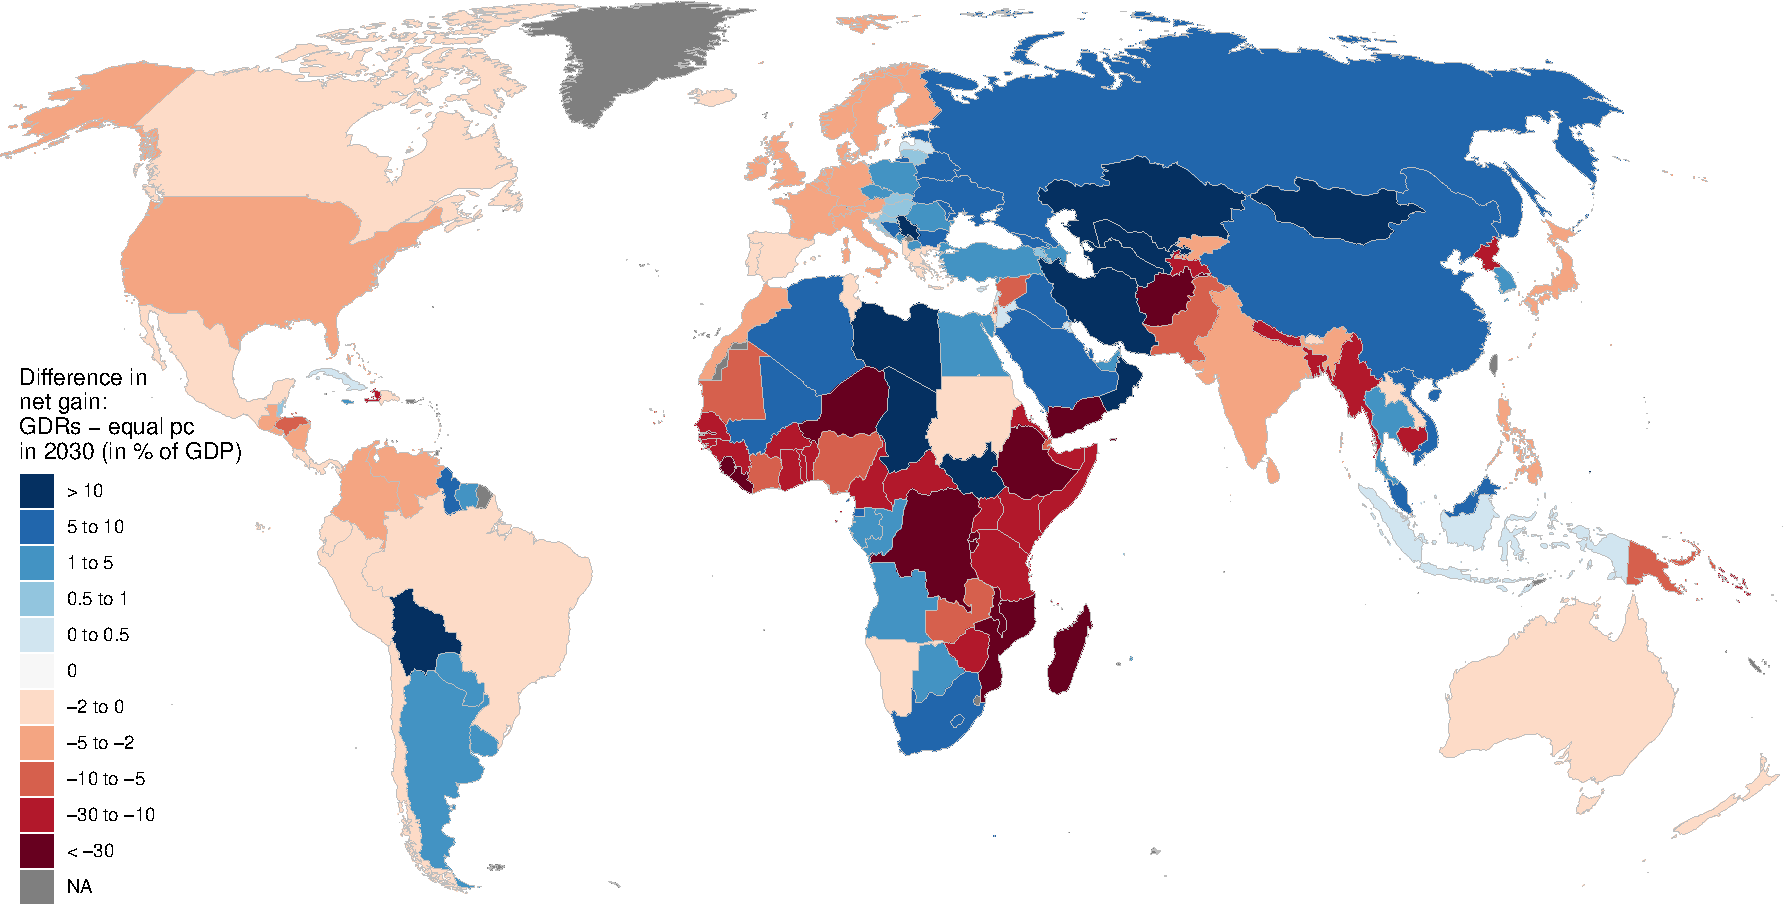
\includegraphics[width=\textwidth]{../figures/maps/diff_gain_gdr_gcs_over_gdp_2030.pdf}} 
    {\small \textit{Note:} GDRs are calibrated with the preferred parameters of the \href{https://usfairshare.org/}{U.S. Climate Action Network} \citep{athanasiou_fair_2022} using the Efficiency scenario (2\textdegree{}C with $>$50\% chance) of the Global Energy Assessment \citep{johansson_global_2012} and a price of \$144/tCO$_\text{2}$.}
\end{figure} % TODO? GDR -> CERF in figure?
